\section{Introducción}
En este trabajo práctico se busca experimentar con el procesamiento con instrucciones SIMD que operan con múltiples datos simultáneamente.\\ 
Con este fin, desarrollamos distintas implementaciones de los filtros Blur, Merge y HSL sobre imágenes y evaluamos su rendimiento.\\
\subsection{Sobre la experimentación}
Realizamos las experimentaciones para los tres filtros con sus respectivas implementaciones de la manera detallada a continuación.\\
Para realizar casos de tests exhaustivos, utilizamos imágenes de distintos tamaños y tipos.
Tomamos imágenes de colores constantes (es decir, imágenes totalmente blancas, azules, verdes, rojas y negras), imágenes que tienden a estos colores e imágenes mixtas.
Cada una de estas imágenes las procesamos en los tamaños 40x40 (1600 píxeles), 300x300 (90000 píxeles) y 600x600 (360000 píxeles), ya que nos pareció una variación razonable para mostrar la performance de las distintas implementaciones de los filtros.\\
Para cada filtro y cada implementación, calculamos la cantidad de ciclos de clock que transcurren en las instrucciones que procesan la imagen (obviando la carga de la misma y el guardado de datos). Para medir los ciclos de clock usamos las funciones provistas por la cátedra en el archivo rdtsc.h. 
Teniendo en cuenta que existen problemáticas al momento de conocer el tiempo de ejecución real de los programas, ya que la ejecución puede ser interrumpida por el scheduler para realizar un cambio de contexto o bien que los procesadores varían la frecuencia de reloj, ideamos la siguiente metodología para medir la cantidad de ciclos de clock de nuestras implementaciones: para cada test entonces, realizamos 100 repeticiones, tomando el promedio de los resultados obtenidos.\\ Luego, descartamos el 10\% de los peores casos. Una vez hecho esto, calculamos el desvío estándar del 90\% de los casos restantes. De esta forma, obtuvimos un resultado promedio, y sumando y restando a este valor el desvío estándar, el resultado esperado en mejor y peor caso. Así mismo, el desvío estándar también nos sirve como indicador de qué tan precisas fueron las mediciones.\\
Además, compilamos las implementaciones de C provistas por la cátedra con el parámetro de compilación -O3, que aseguraba la versión más optimizada del código, para poder acercarnos a la mejor ejecución posible de dichas implementaciones.\\

%TODO: Calcular o chamuyar el desvío estándar en las mediciones y hablar un poco de eso luego.

Cabe destacar que la computadora en la que realizamos las experimentaciones cuenta con las siguientes especificaciones técnicas:\\
%TODO: Agregar características técnicas de la computadora del Mago

Para experimentar acerca de si variaba el rendimiento de una implementación en función del tipo de imagen testeado elaboramos la siguiente estrategia. Agrupamos los distintos tipos de imágenes con los que contábamos como casos de prueba, descritos en la introducción del apartado de experimentación, y tomamos el promedio de tiempos de ejecución (tomando el 10\% peor como outliers) para cada subgrupo. Luego, tomando los promedios de cada tipo de imagen como el representante de dicho tipo, calculamos el desvío estándar entre todos los representantes. Una vez calculado el desvío estándar, lo dividimos por el promedio y multiplicamos por 100 para tener un “porcentaje de desviación”. De esta forma, un porcentaje elevado significa que los representantes de cada tipo de imagen difieren significativamente, mientras que un porcentaje pequeño, que todos los representantes estan cercanos al promedio y por lo tanto, las mediciones dentro de todos los tipos se mantiene estable.\\

Por último, tomamos como decisión para una mayor claridad en los gráficos, el utilizar escala logarítmica para representar los ciclos de clock, ya que de no hacerlo, se perdía claridad y representatividad en los mismos. De cualquier manera, en cada gráfico figurará qué tipo de escala está utilizando, y cualquier otra información relevante.
A continuación, describiremos para cada filtro su desarrolo, los resultados obtenidos y el análisis comparativo en relación con las implementaciones que realizamos y otras posibles.\\\\\\\\\\\\\\\\\\

% \begin{figure}[ht]
% \centering
% 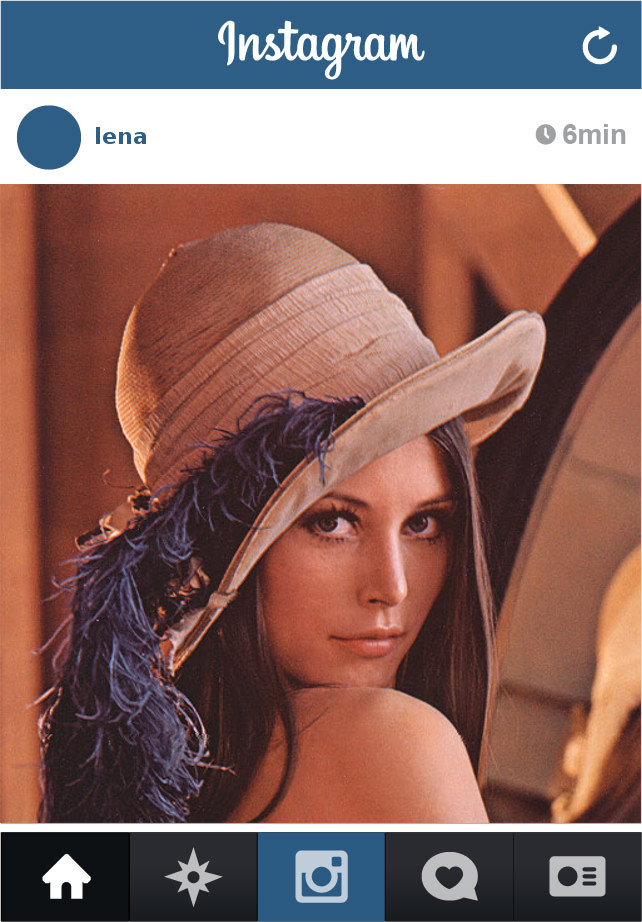
\includegraphics[width=90mm]{introduccion/lena_instagram.jpg}
% %\caption{A simple caption \label{overflow}}
% \end{figure}
